% ---------------------------------------------------------------- 5 setup
\section{Experimental Setup}
\label{sec:setup}

This section describes the data, the model and its parameters, the receivers that are compared, the selection of the decoder, and the protocol under which the results were obtained. The protocol, the primary endpoint, the tests and the equivalence margins were fixed in the project repository before the confirmatory runs. Figure~\ref{fig:floweval} outlines the procedure.

\begin{figure}[!tbp]
\centering
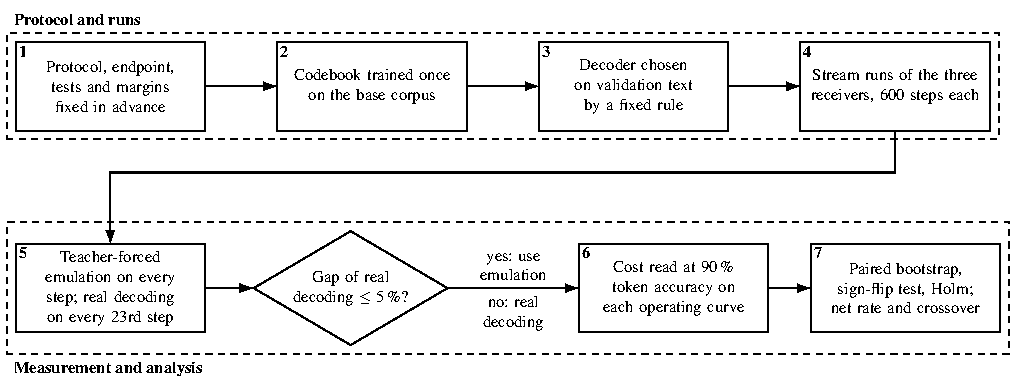
\includegraphics[width=\linewidth]{diagrams/fig_flow_eval.pdf}
\caption{Evaluation procedure. Steps 1 to 3 were completed before the confirmatory stream runs. The decision in the second row is the pre-specified rule that selects the measurement on which the reported costs rest; Section~\ref{sec:setup-protocol} states how it was applied.}
\label{fig:floweval}
\end{figure}

\subsection{Data, Model, and Parameters}
\label{sec:setup-model}

The frozen prior is GPT-2 \cite{radford2019}, with 124,439,808 parameters, a vocabulary of $V = 50{,}257$ tokens and an embedding width of $D = 768$. The codebook uses $M = 16$ real symbols per token, nested at the prefix lengths $\{2,4,6,8,12,16\}$ (shell widths $2|2|2|2|4|4$), with $D_\mathrm{h} = 256$ hidden units and a peak ratio of $\zeta = 4$, which amounts to 213,248 parameters. It was trained once on the base corpus, the Europarl sample distributed with NLTK \cite{koehn2005} (14,006 sentences of 4--30 words, split 80/10/10 by document), for 2000 steps of 256 tokens, of which a quarter were drawn uniformly from the vocabulary, with one SNR per token drawn uniformly in $[\gamma_\mathrm{lo},\gamma_\mathrm{hi}] = [0,20]$\,dB and three prefix lengths per batch, using AdamW with a learning rate of $2\times10^{-3}$, 100 warm-up steps, cosine decay and gradient clipping at 1.0; training took 2194\,s on a CPU.

The drift stream is built from AG News \cite{zhang2015agnews}, with four topic classes, and TeleQnA \cite{maatouk2023teleqna}, a collection of telecommunication questions on standards and research with five categories, restricted to sentences of 4--30 words. An AG News document consists of a title and its description, and a TeleQnA document of a question, its explanation and its answer. The stream visits AG News, TeleQnA, AG News and TeleQnA for $\tau_\mathrm{slow} = 150$ steps each (600 steps), with $N_\mathrm{c} = 6$ parallel conversations, a topic change every $\tau_\mathrm{med} = 30$ steps and $\kappa = 0.9$; a change of domain ends every conversation. One run therefore carries 3600 messages of about 18 tokens. The stream draws its documents from the training split of each corpus, with replacement within a run, while the validation set of Section~\ref{sec:setup-receivers} is drawn from the validation split, so that no validation sentence occurs in the stream. The channel is AWGN with the SNR process~(\ref{eq:snr}) at $\mu_\gamma = 10$\,dB, $\rho = 0.95$ and $\sigma_\gamma = 4$\,dB, clipped to $[0,20]$\,dB.

The context holds up to 48 tokens of the preceding messages of a conversation. The medium memory, consisting of the two fusion weights and $\vect{u}\in\R^{768}$, learns with Adam at a rate of $10^{-3}$ and is shipped every $C_\mathrm{med} = 10$ steps, at a cost of 6257 bits per shipment according to the ledger: 6256 bits for its 770 active entries and a 1-bit flag for an inactive cache-mixing weight that belongs to the same parameter group in the implementation. The slow memory has $K_\mathrm{s} = 2$ LoRA slots of rank $r = 8$ with $\alpha = 16$ on the query--key--value projection of the last six of the twelve layers, that is, 147,456 parameters per slot; it learns with Adam at $5\times10^{-4}$ and is shipped every $C_\mathrm{slow} = 50$ steps at 1,180,032 bits per shipment. The slot is chosen every $C_\mathrm{sel} = 10$ steps with $\delta = 0.05$ bits per token, shipments use $b = 8$ bits per entry, and the adaptation loss~(\ref{eq:adapt-loss}) uses the prefix length of 6 symbols and one further prefix length per step. With these values,~(\ref{eq:syncrate}) gives $\bar{B}_\mathrm{sync} = 625.7 + 23{,}600.6 + 0.2 = 24{,}226.5$ bits per adaptation step, which coincides with the value recorded by the ledger. Table~\ref{tab:params} collects the parameters.

\begin{table}[!tbp]
\centering
\caption{Simulation parameters.}
\label{tab:params}
\footnotesize
\begin{tabular}{@{}p{0.17\linewidth}p{0.40\linewidth}p{0.37\linewidth}@{}}
\toprule
Group & Parameter & Value \\
\midrule
Language prior & Model; parameters & GPT-2 (frozen); 124,439,808 \\
 & Vocabulary $V$; embedding width $D$ & 50,257; 768 \\
Codebook & Symbols per token $M$; prefix lengths $m_k$ & 16; 2, 4, 6, 8, 12, 16 \\
 & Hidden units $D_\mathrm{h}$; peak ratio $\zeta$; parameters & 256; 4; 213,248 \\
 & Training steps; tokens per batch; uniform share & 2000; 256; 25\% \\
 & Training SNR & $\mathcal{U}[0,20]$\,dB per token \\
Stream & Domains, in order & AG News, TeleQnA, AG News, TeleQnA \\
 & $\tau_\mathrm{slow}$; $\tau_\mathrm{med}$; $\kappa$; $N_\mathrm{c}$; steps & 150; 30; 0.9; 6; 600 \\
Channel & Type; $\mu_\gamma$; $\rho$; $\sigma_\gamma$; range & AWGN; 10\,dB; 0.95; 4\,dB; 0--20\,dB \\
Fast memory & Context length & 48 tokens \\
Medium memory & Content; learning rate; period $C_\mathrm{med}$ & $w_\mathrm{p}$, $w_\mathrm{l}$, $\vect{u}\in\R^{768}$; $10^{-3}$; 10 steps \\
Slow memory & Slots $K_\mathrm{s}$; LoRA rank $r$; $\alpha$; layers & 2; 8; 16; last 6 of 12 \\
 & Parameters per slot; learning rate; period $C_\mathrm{slow}$ & 147,456; $5\times10^{-4}$; 50 steps \\
Slot choice & Period $C_\mathrm{sel}$; margin $\delta$; cost & 10 steps; 0.05 bits/token; 2 bits \\
Synchronization & Bits per entry $b$; scale per tensor; per shipment & 8; 32 bits; 6257 (medium), 1,180,032 (slot) \\
Decoder & Beam width $B$; first round $m_{k_0}$; reopening & 4; 6 symbols; no \\
Refinement & Thresholds $\tau$ & 0.5, 0.7, 0.9, 0.95, 0.99 \\
Endpoint & Target token accuracy $A^\star$ & 0.90 \\
\bottomrule
\end{tabular}
\end{table}

\subsection{Compared Receivers and Decoder Selection}
\label{sec:setup-receivers}

Three receivers are compared on the same streams, codebook and decoder: the \emph{frozen} receiver, which decodes every message on its own with the unadapted prior; the \emph{context memory} receiver, which adds the fast memory only and therefore requires no synchronization; and \emph{DN-SC}, with all three memories. Each receiver is evaluated at every fixed prefix length and with selective refinement, and every relative change is stated against the frozen receiver at a fixed prefix, which needs neither signaling nor synchronization. Component ablations, namely single-rate shipping at approximately the same synchronization budget, elastic weight consolidation \cite{kirkpatrick2017}, shipping after every step, and DN-SC without slots, without context or with a single period for both shipped memories, stem from pilot runs of an earlier code version and are reported as exploratory in Section~\ref{sec:results-memories}.

The decoder of the refinement policy was selected on validation text only, by a rule written down before the selection was run. The candidates comprised the first round (2, 4 or 6 symbols per token), the reopening of closed tokens (permitted or not) and the decoding of every pass (greedy, or beam search of width 2 or 4). The validation set contains one sentence, at a random position and with the true preceding sentences of its document as context, from each of 32 documents of the validation splits of AG News, TeleQnA and a public mirror of the News Category Dataset \cite{misra2022}, that is, 96 messages and 1633 tokens, with the frozen prior, one AWGN realization per message and the SNR drawn from the stationary law of the SNR process (mean of the draws 9.8\,dB). The criterion is the number of real symbols per token for 90\% token accuracy under free-running decoding, with the signaling charged at its entropy. The first stage compares the six greedy candidates, counting candidates within 1\% as tied and assigning a tie to the candidate with fewer rounds per message; the second stage adds beam widths 2 and 4 to the winner, and a beam is adopted only if it lowers the criterion by more than 2\%, since it increases computation. Because a beam search changes the receiver, the fixed-prefix reference is decoded with the same beam.

\subsection{Evaluation Protocol and Statistical Analysis}
\label{sec:setup-protocol}

Every message is scored prequentially, with the parameters that the receiver holds before the update of that step. Two measurements are taken. Teacher-forced emulation on every step scores each token given the true preceding tokens, which requires one pass of the language model per step and yields the complete operating curve over all prefix lengths and thresholds; the decisions of the emulated policy at $\tau = 0.9$ are written into the receiver's context. Real decoding on every 23rd step (26 steps and 156 messages per run; 23 is coprime with the shipping periods of 10 and 50 steps, so that the audited steps sample every phase of the shipping cycles) decodes the same received symbols free-running, round by round and with the configured decoder, for selective refinement at every threshold and for every fixed prefix alike. A decision rule fixed in advance determines which measurement constitutes the result: the teacher-forced curves are retained if, on the audited steps, real decoding requires at most 5\% more forward symbols at the target than the emulation for every receiver of the headline table; otherwise the real-decoding figures replace them on both sides of every comparison. The implemented check covered the refinement policy of every receiver, whereas the rule as worded also covers the fixed-prefix receivers of that table, and applied as worded it selects the real-decoding figures (Section~\ref{sec:results-drift}). The article nevertheless quotes the teacher-forced figures as the headline, because they are the more conservative, and reports the real-decoding figures alongside for every receiver; this is a declared deviation from the pre-specified rule.

Two simplifications of the stream simulation are stated explicitly. First, the adaptation loss~(\ref{eq:adapt-loss}) of a step reuses that step's channel realization; because an update reaches the receiver only after the step has been decoded and the noise is independent across steps, this is equivalent in distribution to a realization drawn by the transmitter for the update alone, although the shared realization couples the update weakly with the receiver's context of the next step. Second, every message is transmitted once with the gains~(\ref{eq:gain}) computed over all its tokens, and the refinement rounds, emulated and real alike, are read off that transmission, so that a refinement round carries its shell at the gain of the whole message rather than at the gain of the requested tokens. Section~\ref{sec:results-drift} quantifies the effect of the second simplification.

The frozen receiver and DN-SC were run on seeds 0--5 and the context memory receiver on seeds 0, 3, 4 and 5; its runs on seeds 1 and 2 were interrupted by a restart of the machine and not repeated. Seeds 3--5 had never been run before the protocol was fixed. Seeds 0--2 ran on a Linux server CPU with one thread per run and seeds 3--5 on a Windows~11 laptop CPU with two threads per run, from code revisions whose stream runner and decoder are identical. The seed is the unit of replication. Let $d_j$ denote the relative change of a receiver against the reference on seed $j$ of $n_\mathrm{s}$ seeds. The seed-level test is an exact sign-flip permutation test,
\begin{equation}
p = 2^{-n_\mathrm{s}}\sum_{\vect{\sigma}\in\{-1,1\}^{n_\mathrm{s}}}\mathbb{1}\Bigl\{\Bigl|\sum_{j=1}^{n_\mathrm{s}}\sigma_j d_j\Bigr| \ge \Bigl|\sum_{j=1}^{n_\mathrm{s}} d_j\Bigr|\Bigr\},
\label{eq:signflip}
\end{equation}
whose smallest attainable two-sided value is $2/2^{n_\mathrm{s}}$, that is, 0.031 for six seeds, reached only when all seeds agree in sign, and 0.125 for four seeds. Over the $n_\mathrm{r}$ receivers compared with the reference, the ordered $p$-values are adjusted by the Holm procedure \cite{holm1979},
\begin{equation}
\tilde{p}_{(i)} = \max_{i'\le i}\,\min\bigl\{1,\,(n_\mathrm{r}-i'+1)\,p_{(i')}\bigr\}.
\label{eq:holm}
\end{equation}
For real decoding, the operating curves of the audited steps are pooled over the seeds, every receiver is compared with the frozen receiver on the same seeds and steps, and the 95\% interval of each relative change $\Delta = S(A^\star)/S^\mathrm{ref}(A^\star)-1$ is the percentile interval of $N_\mathrm{b} = 2000$ paired bootstrap replicates $\beta = 1,\dots,N_\mathrm{b}$ \cite{efron1993},
\begin{equation}
\Delta^{*(\beta)} = \frac{S^{*(\beta)}(A^\star)}{S^{\mathrm{ref},*(\beta)}(A^\star)}-1,\qquad
\mathrm{CI}_{95} = \Bigl[\Delta^{*}_{(0.025)},\,\Delta^{*}_{(0.975)}\Bigr],
\label{eq:bootstrap}
\end{equation}
in which the audited steps are resampled in pairs within each seed and a replicate whose curve misses the target counts as an infinite cost. Differences in prior cross-entropy between receivers are given with 95\% block-bootstrap intervals over steps with blocks of 25 steps \cite{kunsch1989}, and a claim of no meaningful difference requires two one-sided tests \cite{schuirmann1987} with the 90\% interval inside $\pm0.05$ bits per token.
